\documentclass[aspectratio=169,11pt]{beamer}

% =========================================================
% Theme
% =========================================================
\usetheme{Madrid}
\usecolortheme{seahorse}
\setbeamertemplate{navigation symbols}{}

% =========================================================
% Packages
% =========================================================
\usepackage[utf8]{inputenc}
\usepackage[T1]{fontenc}
\usepackage{lmodern}
\usepackage{amsmath,amssymb}
\usepackage{xcolor}
\usepackage{booktabs}
\usepackage{array}
\usepackage{listings}
\usepackage{tikz}
\usetikzlibrary{arrows.meta,positioning,fit,calc,shapes.geometric}
\usepackage{hyperref}
\hypersetup{pdfpagemode=UseNone}

% =========================================================
% Colors
% =========================================================
\definecolor{deepblue}{RGB}{0,51,102}
\definecolor{softblue}{RGB}{220,235,247}
\definecolor{softgreen}{RGB}{223,242,228}
\definecolor{softorange}{RGB}{255,238,214}
\definecolor{softred}{RGB}{252,228,228}
\definecolor{codebg}{RGB}{248,248,248}
\definecolor{mygray}{RGB}{90,90,90}
\definecolor{mypurple}{RGB}{102,0,153}

% =========================================================
% Listings
% =========================================================
\lstset{
	language=Java,
	basicstyle=\ttfamily\small,
	backgroundcolor=\color{codebg},
	frame=single,
	breaklines=true,
	columns=fullflexible,
	showstringspaces=false,
	keywordstyle=\color{deepblue}\bfseries,
	commentstyle=\color{green!50!black},
	stringstyle=\color{mypurple},
	numbers=left,
	numberstyle=\tiny\color{mygray},
	stepnumber=1,
	numbersep=8pt
}

% =========================================================
% Title Info
% =========================================================
\title[Week 4 -- Part 3]{Concurrency and Distributed Systems}
\subtitle{Week 4 -- Part 3: Visibility vs Atomicity and Broken Double-Checked Locking}
\author{Dr. Mohamad Aoude}
\institute{Faculty of Engineering}
\date{\today}

% =========================================================
% Custom Blocks
% =========================================================
\setbeamercolor{block title}{bg=deepblue!85, fg=white}
\setbeamercolor{block body}{bg=softblue, fg=black}

\setbeamercolor{alertblock title}{bg=red!75!black, fg=white}
\setbeamercolor{alertblock body}{bg=softred, fg=black}

\setbeamercolor{exampleblock title}{bg=green!50!black, fg=white}
\setbeamercolor{exampleblock body}{bg=softgreen, fg=black}

% =========================================================
% Footer
% =========================================================
\setbeamertemplate{footline}{
	\leavevmode
	\hbox{
		\begin{beamercolorbox}[wd=.78\paperwidth,ht=2.5ex,dp=1.2ex,leftskip=0.3cm]{author in head/foot}
			\usebeamerfont{author in head/foot}Concurrency and Distributed Systems --- Week 4 Part 3
		\end{beamercolorbox}
		\begin{beamercolorbox}[wd=.22\paperwidth,ht=2.5ex,dp=1.2ex,rightskip=0.3cm]{date in head/foot}
			\hfill \insertframenumber/\inserttotalframenumber
		\end{beamercolorbox}
	}
}

% =========================================================
% Document
% =========================================================
\begin{document}
	
	% =========================================================
	\begin{frame}
		\titlepage
	\end{frame}
	
	% =========================================================
	\begin{frame}{Part 3 Roadmap}
		\tableofcontents
	\end{frame}
	
	\section{From Visibility to Atomicity}
	\section{The Lost Update Problem}
	\section{Why volatile Is Not Enough}
	\section{Connecting Back to Week 3}
	\section{Broken Double-Checked Locking}
	\section{Fixing DCL with volatile}
	\section{Safer Alternatives and Lab Preparation}
	
	% =========================================================
	\begin{frame}{Where We Are in Week 4}
		\begin{block}{Part 1}
			We learned why stale reads and visibility problems occur.
		\end{block}
		
		\vspace{0.2cm}
		
		\begin{block}{Part 2}
			We learned that \texttt{volatile} provides:
			\begin{itemize}
				\item visibility
				\item ordering guarantees
				\item happens-before through volatile communication
			\end{itemize}
		\end{block}
		
		\vspace{0.2cm}
		
		\begin{alertblock}{Part 3 challenge}
			A program can still be wrong even when visibility is correct.
		\end{alertblock}
		
		\vspace{0.2cm}
		
		\begin{exampleblock}{Main question}
			If threads can see updates correctly, why can the result still be incorrect?
		\end{exampleblock}
	\end{frame}
	
	% =========================================================
	\begin{frame}{Learning Objectives}
		By the end of this lecture, students should be able to:
		
		\begin{itemize}
			\item distinguish sharply between \textbf{visibility} and \textbf{atomicity}
			\item explain why \texttt{counter++} is not atomic
			\item analyze the lost update problem
			\item understand why locks from Week 3 are still relevant
			\item explain why broken double-checked locking was historically unsafe
			\item explain why \texttt{volatile} is required for correct DCL in modern Java
			\item identify safer alternatives to DCL
		\end{itemize}
	\end{frame}
	
	% =========================================================
	\begin{frame}{Visibility vs Atomicity}
		\begin{columns}[T]
			\column{0.48\textwidth}
			\begin{block}{Visibility}
				Can one thread see another thread's update?
			\end{block}
			
			\vspace{0.2cm}
			
			Examples:
			\begin{itemize}
				\item stop flag
				\item ready flag
				\item state publication
			\end{itemize}
			
			\column{0.48\textwidth}
			\begin{block}{Atomicity}
				Does a multi-step operation behave like one indivisible action?
			\end{block}
			
			\vspace{0.2cm}
			
			Examples:
			\begin{itemize}
				\item increment
				\item check-then-act
				\item initialize once
			\end{itemize}
		\end{columns}
		
		\vspace{0.35cm}
		
		\begin{alertblock}{Critical distinction}
			A value can be perfectly visible and still be updated incorrectly.
		\end{alertblock}
	\end{frame}
	
	% =========================================================
	\begin{frame}[fragile]{The Trap: A Volatile Counter}
		\begin{lstlisting}
			class VolatileCounter {
				static volatile int counter = 0;
				
				static void increment() {
					counter++;
				}
			}
		\end{lstlisting}
		
		\vspace{0.2cm}
		
		At first glance, students may think:
		
		\begin{itemize}
			\item the field is shared
			\item the field is volatile
			\item therefore updates are safe
		\end{itemize}
		
		\vspace{0.25cm}
		
		\begin{alertblock}{Wrong}
			\texttt{volatile} does not make \texttt{counter++} atomic.
		\end{alertblock}
	\end{frame}
	
	% =========================================================
	\begin{frame}[fragile]{Why \texttt{counter++} Is Not One Action}
		Conceptually, this statement:
		
		\[
		\texttt{counter++}
		\]
		
		expands into:
		
		\begin{lstlisting}
			int temp = counter;
			temp = temp + 1;
			counter = temp;
		\end{lstlisting}
		
		\vspace{0.3cm}
		
		This is a sequence of steps:
		\begin{enumerate}
			\item read current value
			\item compute new value
			\item write new value
		\end{enumerate}
		
		\vspace{0.3cm}
		
		\begin{alertblock}{Atomicity problem}
			Another thread can interleave between these steps.
		\end{alertblock}
	\end{frame}
	
	% =========================================================
	\begin{frame}[fragile]{Lost Update Example}
		\begin{lstlisting}
			class CounterDemo {
				static int counter = 0;
				
				public static void main(String[] args) throws Exception {
					Thread t1 = new Thread(() -> {
						for (int i = 0; i < 100000; i++) counter++;
					});
					
					Thread t2 = new Thread(() -> {
						for (int i = 0; i < 100000; i++) counter++;
					});
					
					t1.start();
					t2.start();
					t1.join();
					t2.join();
					
					System.out.println(counter);
				}
			}
		\end{lstlisting}
	\end{frame}
	
	% =========================================================
	\begin{frame}{What Result Do We Expect?}
		If both threads increment 100000 times, we expect:
		
		\[
		200000
		\]
		
		\vspace{0.35cm}
		
		But often the observed result is smaller.
		
		\vspace{0.35cm}
		
		\begin{alertblock}{Why?}
			Because two increments can overlap and one update can overwrite another.
		\end{alertblock}
		
		\vspace{0.25cm}
		
		\begin{exampleblock}{This is called a lost update}
			One thread's work is effectively erased by another thread's write.
		\end{exampleblock}
	\end{frame}
	
	% =========================================================
	\begin{frame}{Lost Update Timeline}
		\centering
		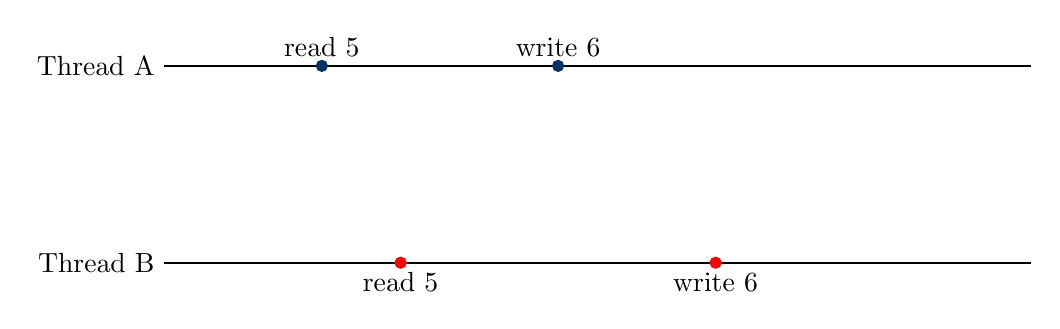
\begin{tikzpicture}[x=1cm,y=1cm]
			\draw[thick] (0,4) -- (11,4);
			\node[left] at (0,4) {Thread A};
			
			\draw[thick] (0,1.5) -- (11,1.5);
			\node[left] at (0,1.5) {Thread B};
			
			\filldraw[deepblue] (2,4) circle (2pt);
			\node[above] at (2,4) {read 5};
			
			\filldraw[deepblue] (5,4) circle (2pt);
			\node[above] at (5,4) {write 6};
			
			\filldraw[red] (3,1.5) circle (2pt);
			\node[below] at (3,1.5) {read 5};
			
			\filldraw[red] (7,1.5) circle (2pt);
			\node[below] at (7,1.5) {write 6};
			
		\end{tikzpicture}
		
		\vspace{0.35cm}
		
		\begin{block}{What happened?}
			Both threads read the same old value 5.  
			Both compute 6.  
			Both write 6.  
			One increment disappears.
		\end{block}
	\end{frame}
	
	% =========================================================
	\begin{frame}[fragile]{Why volatile Still Fails Here}
		Suppose we change:
		
		\begin{lstlisting}
			static int counter = 0;
		\end{lstlisting}
		
		to:
		
		\begin{lstlisting}
			static volatile int counter = 0;
		\end{lstlisting}
		
		\vspace{0.3cm}
		
		Now:
		\begin{itemize}
			\item reads are visible
			\item writes are visible
		\end{itemize}
		
		\vspace{0.3cm}
		
		\begin{alertblock}{But}
			The full read-modify-write sequence is still not one indivisible operation.
		\end{alertblock}
		
		\vspace{0.25cm}
		
		\begin{exampleblock}{Conclusion}
			\texttt{volatile} fixes communication visibility, not compound update safety.
		\end{exampleblock}
	\end{frame}
	
	% =========================================================
	\begin{frame}{This Is the Boundary of volatile}
		\begin{center}
			\begin{tabular}{>{\bfseries}m{3cm} m{6.7cm}}
				What \texttt{volatile} solves & seeing updated values, publication ordering \\
				What \texttt{volatile} does not solve & increment races, check-then-act races, multi-step consistency \\
			\end{tabular}
		\end{center}
		
		\vspace{0.4cm}
		
		\begin{alertblock}{Best teaching sentence}
			\texttt{volatile} tells threads to \textbf{see}.  
			It does not force updates to happen as \textbf{one step}.
		\end{alertblock}
	\end{frame}
	
	% =========================================================
	\begin{frame}{Connecting Back to Week 3}
		In Week 3, we studied:
		\begin{itemize}
			\item \texttt{synchronized}
			\item \texttt{ReentrantLock}
		\end{itemize}
		
		These mechanisms solve a different problem:
		\begin{itemize}
			\item mutual exclusion
			\item protected critical sections
			\item atomic behavior for grouped operations
		\end{itemize}
		
		\vspace{0.35cm}
		
		\begin{exampleblock}{Why this matters now}
			When the problem is:
			\[
			\texttt{``Only one thread must perform this update at a time''}
			\]
			then Week 3 tools remain essential.
		\end{exampleblock}
	\end{frame}
	
	% =========================================================
	\begin{frame}{Week 3 vs Week 4 Tools}
		\centering
		\begin{tabular}{>{\bfseries}m{3cm} >{\centering\arraybackslash}m{2cm} >{\centering\arraybackslash}m{2cm} >{\centering\arraybackslash}m{2cm}}
			\toprule
			Mechanism & Visibility & Ordering & Atomicity \\
			\midrule
			Plain field & No guarantee & No guarantee & No \\
			\texttt{volatile} & Yes & Yes & No \\
			\texttt{synchronized} & Yes & Yes & Yes \\
			\texttt{ReentrantLock} & Yes & Yes & Yes \\
			\bottomrule
		\end{tabular}
		
		\vspace{0.4cm}
		
		\begin{block}{Interpretation}
			Different tools solve different concurrency dimensions.  
			They are not interchangeable.
		\end{block}
	\end{frame}
	
	% =========================================================
	\begin{frame}{Now the Famous Example: Double-Checked Locking}
		Why do programmers attempt double-checked locking (DCL)?
		
		\vspace{0.25cm}
		
		Goal:
		\begin{itemize}
			\item avoid constructing an object more than once
			\item avoid locking after initialization is already done
		\end{itemize}
		
		\vspace{0.25cm}
		
		Typical use case:
		\begin{itemize}
			\item singleton initialization
			\item lazy creation of expensive shared objects
		\end{itemize}
		
		\vspace{0.35cm}
		
		\begin{exampleblock}{Basic idea}
			Check once without locking.  
			If needed, lock and check again before creating.
		\end{exampleblock}
	\end{frame}
	
	% =========================================================
	\begin{frame}[fragile]{Broken Double-Checked Locking}
		\begin{lstlisting}
			class Singleton {
				private static Singleton instance;
				
				static Singleton getInstance() {
					if (instance == null) {
						synchronized (Singleton.class) {
							if (instance == null) {
								instance = new Singleton();
							}
						}
					}
					return instance;
				}
			}
		\end{lstlisting}
	\end{frame}
	
	% =========================================================
	\begin{frame}{Why This Looks Reasonable}
		Students often see the code and think:
		
		\begin{itemize}
			\item outer check avoids unnecessary locking
			\item inner check prevents duplicate creation
			\item synchronized protects construction
			\item therefore the code must be safe
		\end{itemize}
		
		\vspace{0.3cm}
		
		\begin{alertblock}{But historically this was broken}
			The issue is not just mutual exclusion.  
			The issue is also \textbf{safe publication} and \textbf{reordering}.
		\end{alertblock}
	\end{frame}
	
	% =========================================================
	\begin{frame}{Object Creation Is Not One Magical Step}
		This line:
		
		\[
		\texttt{instance = new Singleton();}
		\]
		
		is easy to read as a single action, but conceptually it may involve:
		
		\begin{enumerate}
			\item allocate memory
			\item initialize the object
			\item assign the reference to \texttt{instance}
		\end{enumerate}
		
		\vspace{0.35cm}
		
		\begin{alertblock}{Danger}
			If the reference becomes visible before initialization is fully complete, another thread may observe a non-null but incompletely initialized object.
		\end{alertblock}
	\end{frame}
	
	% =========================================================
	\begin{frame}{Why Reordering Matters in DCL}
		A thread could observe:
		
		\begin{itemize}
			\item \texttt{instance != null}
			\item and therefore skip synchronization
			\item but still receive an object whose construction is not safely published
		\end{itemize}
		
		\vspace{0.35cm}
		
		\begin{exampleblock}{This is subtle}
			The lock protects mutual exclusion during creation, but the outer unsynchronized read still needs correct visibility and ordering guarantees.
		\end{exampleblock}
		
		\vspace{0.25cm}
		
		\begin{alertblock}{Core lesson}
			DCL is not just a lock problem.  
			It is also a memory publication problem.
		\end{alertblock}
	\end{frame}
	
	% =========================================================
	\begin{frame}{A Timeline View of the DCL Risk}
		\centering
		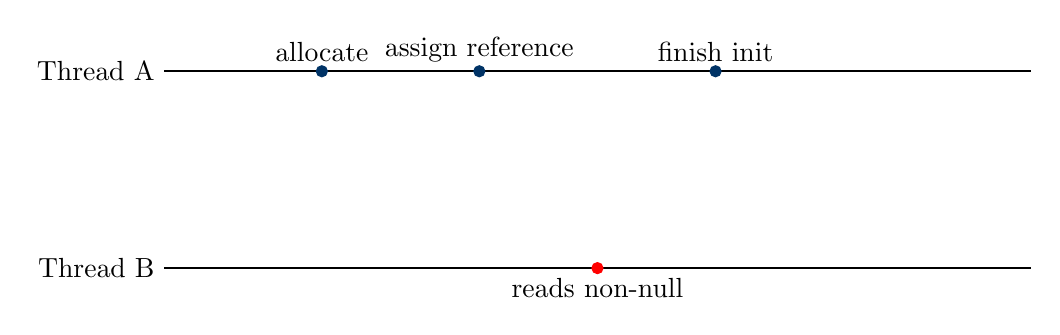
\begin{tikzpicture}[x=1cm,y=1cm]
			\draw[thick] (0,4) -- (11,4);
			\node[left] at (0,4) {Thread A};
			
			\draw[thick] (0,1.5) -- (11,1.5);
			\node[left] at (0,1.5) {Thread B};
			
			\filldraw[deepblue] (2,4) circle (2pt);
			\node[above] at (2,4) {allocate};
			
			\filldraw[deepblue] (4,4) circle (2pt);
			\node[above] at (4,4) {assign reference};
			
			\filldraw[deepblue] (7,4) circle (2pt);
			\node[above] at (7,4) {finish init};
			
			\filldraw[red] (5.5,1.5) circle (2pt);
			\node[below] at (5.5,1.5) {reads non-null};
			
		\end{tikzpicture}
		
		\vspace{0.35cm}
		
		\begin{alertblock}{Interpretation}
			Thread B may observe the shared reference after assignment but before safe initialization is guaranteed to be visible.
		\end{alertblock}
	\end{frame}
	
	% =========================================================
	\begin{frame}[fragile]{Correct DCL with volatile}
		\begin{lstlisting}
			class Singleton {
				private static volatile Singleton instance;
				
				static Singleton getInstance() {
					if (instance == null) {
						synchronized (Singleton.class) {
							if (instance == null) {
								instance = new Singleton();
							}
						}
					}
					return instance;
				}
			}
		\end{lstlisting}
	\end{frame}
	
	% =========================================================
	\begin{frame}{Why volatile Fixes the Publication Side}
		With:
		
		\[
		\texttt{private static volatile Singleton instance;}
		\]
		
		the field now has:
		\begin{itemize}
			\item visibility guarantees
			\item ordering guarantees relevant to publication
		\end{itemize}
		
		\vspace{0.35cm}
		
		\begin{block}{Meaning}
			Once one thread publishes the initialized instance through the volatile field, later readers of that field see a correctly published object.
		\end{block}
		
		\vspace{0.25cm}
		
		\begin{exampleblock}{Division of roles}
			\begin{itemize}
				\item \texttt{synchronized} prevents duplicate construction
				\item \texttt{volatile} prevents unsafe publication / harmful reordering
			\end{itemize}
		\end{exampleblock}
	\end{frame}
	
	% =========================================================
	\begin{frame}{What DCL Teaches Students}
		DCL is a powerful teaching example because it combines:
		
		\begin{itemize}
			\item mutual exclusion
			\item visibility
			\item ordering
			\item publication correctness
			\item performance motivation
		\end{itemize}
		
		\vspace{0.35cm}
		
		\begin{alertblock}{Most important lesson}
			A lock can protect a critical section, but a shared reference still needs correct publication semantics when read outside the lock.
		\end{alertblock}
	\end{frame}
	
	% =========================================================
	\begin{frame}{Should Students Use DCL Often?}
		My opinion: \textbf{usually no}.
		
		\vspace{0.3cm}
		
		Even though DCL is correct in modern Java with \texttt{volatile}, it is still:
		
		\begin{itemize}
			\item subtle
			\item easy to misunderstand
			\item often less clear than safer alternatives
		\end{itemize}
		
		\vspace{0.35cm}
		
		\begin{exampleblock}{Teach DCL for understanding}
			Teach it because it reveals deep concurrency ideas, not because it should be the default design pattern everywhere.
		\end{exampleblock}
	\end{frame}
	
	% =========================================================
	\begin{frame}[fragile]{Safer Alternative: Initialization-on-Demand Holder}
		\begin{lstlisting}
			class Singleton {
				private Singleton() {}
				
				private static class Holder {
					static final Singleton INSTANCE = new Singleton();
				}
				
				static Singleton getInstance() {
					return Holder.INSTANCE;
				}
			}
		\end{lstlisting}
		
		\vspace{0.25cm}
		
		\begin{block}{Why this is attractive}
			It is simpler, cleaner, and avoids many DCL subtleties.
		\end{block}
	\end{frame}
	
	% =========================================================
	\begin{frame}[fragile]{Another Alternative: Eager Initialization}
		\begin{lstlisting}
			class Singleton {
				private static final Singleton INSTANCE = new Singleton();
				
				private Singleton() {}
				
				static Singleton getInstance() {
					return INSTANCE;
				}
			}
		\end{lstlisting}
		
		\vspace{0.25cm}
		
		\begin{exampleblock}{Use when appropriate}
			If lazy creation is not necessary, eager initialization is often the cleanest option.
		\end{exampleblock}
	\end{frame}
	
	% =========================================================
	\begin{frame}{Part 3 Comparison Summary}
		\centering
		\begin{tabular}{>{\bfseries}m{3.2cm} m{6.8cm}}
			Visibility problem & one thread may not see another thread's write \\
			Atomicity problem & a multi-step update can interleave with another thread \\
			\texttt{volatile} helps with & visibility and ordering \\
			\texttt{volatile} does not help with & compound update atomicity \\
			DCL needs & both exclusion and safe publication \\
		\end{tabular}
	\end{frame}
	
	% =========================================================
	\begin{frame}{Common Misconceptions to Kill Here}
		Students should \textbf{not} leave this lecture believing:
		
		\begin{itemize}
			\item ``If a field is volatile, increment is safe''
			\item ``If there is a synchronized block somewhere, publication is automatically safe everywhere''
			\item ``Object construction is one indivisible machine step''
			\item ``DCL is just a fancy lock optimization''
		\end{itemize}
		
		\vspace{0.35cm}
		
		\begin{alertblock}{Replace with}
			\begin{quote}
				Correct concurrent design must separately reason about visibility, ordering, atomicity, and publication.
			\end{quote}
		\end{alertblock}
	\end{frame}
	
	% =========================================================
	\begin{frame}{Lab Preparation for Part 3}
		\begin{block}{Lab 4.5 --- Lost Update Counter}
			Students compare:
			\begin{itemize}
				\item plain \texttt{int}
				\item \texttt{volatile int}
				\item synchronized counter from Week 3
			\end{itemize}
			and explain the differences.
		\end{block}
		
		\vspace{0.25cm}
		
		\begin{block}{Lab 4.6 --- Broken DCL Analysis}
			Students inspect DCL and explain why it is not only a locking issue.
		\end{block}
		
		\vspace{0.25cm}
		
		\begin{block}{Lab 4.7 --- Fix DCL}
			Students add \texttt{volatile} and explain exactly what it contributes.
		\end{block}
	\end{frame}
	
	% =========================================================
	\begin{frame}{Discussion Questions}
		\begin{enumerate}
			\item Why does \texttt{volatile} fail for \texttt{counter++}?
			\item What exactly is lost in a lost-update race?
			\item Why are Week 3 locks still relevant in Week 4?
			\item Why is DCL not just about preventing duplicate construction?
			\item What role does \texttt{volatile} play in correct DCL?
			\item Why might a simpler singleton pattern be preferable?
		\end{enumerate}
	\end{frame}
	
	% =========================================================
	\begin{frame}{Takeaway}
		\begin{alertblock}{Final takeaway for Part 3}
			A concurrent program can have correct visibility and still be wrong because visibility is not the same as atomicity.
		\end{alertblock}
		
		\vspace{0.35cm}
		
		\begin{block}{And}
			Double-checked locking teaches that concurrency correctness is also about safe publication, not only critical-section protection.
		\end{block}
		
		\vspace{0.35cm}
		
		\begin{exampleblock}{Bridge to Part 4}
			Now that we know \texttt{volatile} is not enough for atomic increments, the next question becomes:
			
			\begin{center}
				\Large
				How can we perform atomic updates without using a traditional lock?
			\end{center}
		\end{exampleblock}
		
		\vspace{0.2cm}
		
		That leads directly to:
		\[
		\texttt{AtomicInteger}, \quad \text{CAS}, \quad \text{lock-free programming}
		\]
	\end{frame}
	
	% =========================================================
	\begin{frame}{End of Part 3}
		\centering
		\Huge Questions?
	\end{frame}
	
	% =========================================================
\end{document}